\subsection{N-Hat $\left(\hat{N}\right)$}
Starting with the definition of $\hat{T}(t)$,
\begin{align*}
	\hat{T}(t) &= \frac{\vec{r^\prime}(t)}{v(t)} \\
	\vec{r^{\prime}}(t) &= v(t)\hat{T}(t) \\
	\vec{r^{\prime\prime}}(t) &= v(t)\hat{T}^{\prime}(t)+\hat{T}(t)v^{\prime}(t).
\end{align*}

\noindent
We will show that $\hat{T}(t) \perp \hat{T}^{\prime}(t)$.
\begin{align*}
	\frac{1}{2}\dd{}{t}\left(\hat{T}(t)\cdot\hat{T}(t)\right) &= \hat{T}\cdot\hat{T}^{\prime}(t) \\
	\dd{}{t}\left(\hat{T}\cdot\hat{T}\right) &= \dd{}{t}1 = 0.
\end{align*}
So,
\begin{align*}
	\hat{T}\cdot\hat{T}^{\prime}(t) &= 0 \implies \hat{T}(t) \perp \hat{T}^{\prime}(t) \\
	\hat{N}(t) &= \frac{\hat{T}^{\prime}(t)}{\norm{\hat{T}^{\prime}(t)}}\perp\hat{T}.
\end{align*}

\noindent
$\hat{N}$ is a unit vector perpendicular to $\hat{T}$ that points in the direction that the curve curls into.
It is called the normal vector because it is perpendicular to the curve.
It is in the same plane as $\vec{r}^\prime$, $\hat{T}$, and  $\vec{r}^{\prime\prime}$.

\begin{figure}[H]
	\label{that_nhat}
	\centering
	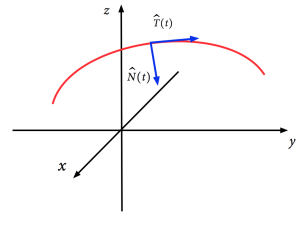
\includegraphics[width = 0.5\textwidth]{./vectorValuedFunctions/TN.PNG}
	\caption{$\hat{T}$ and $\hat{N}$}
\end{figure}

\noindent
$\hat{N}$ allows us to rewrite $\vec{r}^{\prime\prime}$.\\
\begin{equation*}
	\vec{r}^{\prime\prime}(t)=\frac{\mathrm{d}v}{\mathrm{d}t}\hat{T}(t)+v^{2}(t)\kappa(t)\hat{N}(t)
\end{equation*}

\noindent
We can see that $\vec{r}^{\prime\prime}(t)$ has two parts. If $\vec{r}(t)$ represents position, then $\frac{\mathrm{d}v}{\mathrm{d}t}$ represents linear acceleration and $v^2(t)\kappa(t)$ represents centripetal acceleration.
You might recognize the formula for centripetal acceleration in the 2nd part from physics.
If we let $R(t) = \frac{1}{\kappa(t)}$, then the 2nd part becomes $\frac{v^2(t)}{R(t)}$, which looks exactly like the formula for centripetal acceleration for uniform circular motion: $a_c = \frac{v^2}{r}$.